%% bare_jrnl.tex
%% V1.4b
%% 2015/08/26
%% by Michael Shell
%% see http://www.michaelshell.org/
%% for current contact information.
%%
%% This is a skeleton file demonstrating the use of IEEEtran.cls
%% (requires IEEEtran.cls version 1.8b or later) with an IEEE
%% journal paper.
%%
%% Support sites:
%% http://www.michaelshell.org/tex/ieeetran/
%% http://www.ctan.org/pkg/ieeetran
%% and
%% http://www.ieee.org/

%%*************************************************************************
%% Legal Notice:
%% This code is offered as-is without any warranty either expressed or
%% implied; without even the implied warranty of MERCHANTABILITY or
%% FITNESS FOR A PARTICULAR PURPOSE! 
%% User assumes all risk.
%% In no event shall the IEEE or any contributor to this code be liable for
%% any damages or losses, including, but not limited to, incidental,
%% consequential, or any other damages, resulting from the use or misuse
%% of any information contained here.
%%
%% All comments are the opinions of their respective authors and are not
%% necessarily endorsed by the IEEE.
%%
%% This work is distributed under the LaTeX Project Public License (LPPL)
%% ( http://www.latex-project.org/ ) version 1.3, and may be freely used,
%% distributed and modified. A copy of the LPPL, version 1.3, is included
%% in the base LaTeX documentation of all distributions of LaTeX released
%% 2003/12/01 or later.
%% Retain all contribution notices and credits.
%% ** Modified files should be clearly indicated as such, including  **
%% ** renaming them and changing author support contact information. **
%%*************************************************************************


% *** Authors should verify (and, if needed, correct) their LaTeX system  ***
% *** with the testflow diagnostic prior to trusting their LaTeX platform ***
% *** with production work. The IEEE's font choices and paper sizes can   ***
% *** trigger bugs that do not appear when using other class files.       ***                          ***
% The testflow support page is at:
% http://www.michaelshell.org/tex/testflow/



\documentclass[journal, onecolumn]{IEEEtran}
%
% If IEEEtran.cls has not been installed into the LaTeX system files,
% manually specify the path to it like:
% \documentclass[journal]{../sty/IEEEtran}





% Some very useful LaTeX packages include:
% (uncomment the ones you want to load)


% *** MISC UTILITY PACKAGES ***
%
%\usepackage{ifpdf}
% Heiko Oberdiek's ifpdf.sty is very useful if you need conditional
% compilation based on whether the output is pdf or dvi.
% usage:
% \ifpdf
%   % pdf code
% \else
%   % dvi code
% \fi
% The latest version of ifpdf.sty can be obtained from:
% http://www.ctan.org/pkg/ifpdf
% Also, note that IEEEtran.cls V1.7 and later provides a builtin
% \ifCLASSINFOpdf conditional that works the same way.
% When switching from latex to pdflatex and vice-versa, the compiler may
% have to be run twice to clear warning/error messages.






% *** CITATION PACKAGES ***
%
%\usepackage{cite}
% cite.sty was written by Donald Arseneau
% V1.6 and later of IEEEtran pre-defines the format of the cite.sty package
% \cite{} output to follow that of the IEEE. Loading the cite package will
% result in citation numbers being automatically sorted and properly
% "compressed/ranged". e.g., [1], [9], [2], [7], [5], [6] without using
% cite.sty will become [1], [2], [5]--[7], [9] using cite.sty. cite.sty's
% \cite will automatically add leading space, if needed. Use cite.sty's
% noadjust option (cite.sty V3.8 and later) if you want to turn this off
% such as if a citation ever needs to be enclosed in parenthesis.
% cite.sty is already installed on most LaTeX systems. Be sure and use
% version 5.0 (2009-03-20) and later if using hyperref.sty.
% The latest version can be obtained at:
% http://www.ctan.org/pkg/cite
% The documentation is contained in the cite.sty file itself.






% *** GRAPHICS RELATED PACKAGES ***
%
\ifCLASSINFOpdf
  % \usepackage[pdftex]{graphicx}
  % declare the path(s) where your graphic files are
  % \graphicspath{{../pdf/}{../jpeg/}}
  % and their extensions so you won't have to specify these with
  % every instance of \includegraphics
  % \DeclareGraphicsExtensions{.pdf,.jpeg,.png}
\else
  % or other class option (dvipsone, dvipdf, if not using dvips). graphicx
  % will default to the driver specified in the system graphics.cfg if no
  % driver is specified.
  % \usepackage[dvips]{graphicx}
  % declare the path(s) where your graphic files are
  % \graphicspath{{../eps/}}
  % and their extensions so you won't have to specify these with
  % every instance of \includegraphics
  % \DeclareGraphicsExtensions{.eps}
\fi
% graphicx was written by David Carlisle and Sebastian Rahtz. It is
% required if you want graphics, photos, etc. graphicx.sty is already
% installed on most LaTeX systems. The latest version and documentation
% can be obtained at: 
% http://www.ctan.org/pkg/graphicx
% Another good source of documentation is "Using Imported Graphics in
% LaTeX2e" by Keith Reckdahl which can be found at:
% http://www.ctan.org/pkg/epslatex
%
% latex, and pdflatex in dvi mode, support graphics in encapsulated
% postscript (.eps) format. pdflatex in pdf mode supports graphics
% in .pdf, .jpeg, .png and .mps (metapost) formats. Users should ensure
% that all non-photo figures use a vector format (.eps, .pdf, .mps) and
% not a bitmapped formats (.jpeg, .png). The IEEE frowns on bitmapped formats
% which can result in "jaggedy"/blurry rendering of lines and letters as
% well as large increases in file sizes.
%
% You can find documentation about the pdfTeX application at:
% http://www.tug.org/applications/pdftex





% *** MATH PACKAGES ***
%
\usepackage{amsmath}
\usepackage{amssymb}
\usepackage{booktabs}
\usepackage{tikz}
\usetikzlibrary{positioning,shapes,arrows}
% A popular package from the American Mathematical Society that provides
% many useful and powerful commands for dealing with mathematics.
%
% Note that the amsmath package sets \interdisplaylinepenalty to 10000
% thus preventing page breaks from occurring within multiline equations. Use:
%\interdisplaylinepenalty=2500
% after loading amsmath to restore such page breaks as IEEEtran.cls normally
% does. amsmath.sty is already installed on most LaTeX systems. The latest
% version and documentation can be obtained at:
% http://www.ctan.org/pkg/amsmath





% *** SPECIALIZED LIST PACKAGES ***
%
%\usepackage{algorithmic}
% algorithmic.sty was written by Peter Williams and Rogerio Brito.
% This package provides an algorithmic environment fo describing algorithms.
% You can use the algorithmic environment in-text or within a figure
% environment to provide for a floating algorithm. Do NOT use the algorithm
% floating environment provided by algorithm.sty (by the same authors) or
% algorithm2e.sty (by Christophe Fiorio) as the IEEE does not use dedicated
% algorithm float types and packages that provide these will not provide
% correct IEEE style captions. The latest version and documentation of
% algorithmic.sty can be obtained at:
% http://www.ctan.org/pkg/algorithms
% Also of interest may be the (relatively newer and more customizable)
% algorithmicx.sty package by Szasz Janos:
% http://www.ctan.org/pkg/algorithmicx




% *** ALIGNMENT PACKAGES ***
%
%\usepackage{array}
% Frank Mittelbach's and David Carlisle's array.sty patches and improves
% the standard LaTeX2e array and tabular environments to provide better
% appearance and additional user controls. As the default LaTeX2e table
% generation code is lacking to the point of almost being broken with
% respect to the quality of the end results, all users are strongly
% advised to use an enhanced (at the very least that provided by array.sty)
% set of table tools. array.sty is already installed on most systems. The
% latest version and documentation can be obtained at:
% http://www.ctan.org/pkg/array


% IEEEtran contains the IEEEeqnarray family of commands that can be used to
% generate multiline equations as well as matrices, tables, etc., of high
% quality.




% *** SUBFIGURE PACKAGES ***
%\ifCLASSOPTIONcompsoc
%  \usepackage[caption=false,font=normalsize,labelfont=sf,textfont=sf]{subfig}
%\else
%  \usepackage[caption=false,font=footnotesize]{subfig}
%\fi
% subfig.sty, written by Steven Douglas Cochran, is the modern replacement
% for subfigure.sty, the latter of which is no longer maintained and is
% incompatible with some LaTeX packages including fixltx2e. However,
% subfig.sty requires and automatically loads Axel Sommerfeldt's caption.sty
% which will override IEEEtran.cls' handling of captions and this will result
% in non-IEEE style figure/table captions. To prevent this problem, be sure
% and invoke subfig.sty's "caption=false" package option (available since
% subfig.sty version 1.3, 2005/06/28) as this is will preserve IEEEtran.cls
% handling of captions.
% Note that the Computer Society format requires a larger sans serif font
% than the serif footnote size font used in traditional IEEE formatting
% and thus the need to invoke different subfig.sty package options depending
% on whether compsoc mode has been enabled.
%
% The latest version and documentation of subfig.sty can be obtained at:
% http://www.ctan.org/pkg/subfig




% *** FLOAT PACKAGES ***
%
%\usepackage{fixltx2e}
% fixltx2e, the successor to the earlier fix2col.sty, was written by
% Frank Mittelbach and David Carlisle. This package corrects a few problems
% in the LaTeX2e kernel, the most notable of which is that in current
% LaTeX2e releases, the ordering of single and double column floats is not
% guaranteed to be preserved. Thus, an unpatched LaTeX2e can allow a
% single column figure to be placed prior to an earlier double column
% figure.
% Be aware that LaTeX2e kernels dated 2015 and later have fixltx2e.sty's
% corrections already built into the system in which case a warning will
% be issued if an attempt is made to load fixltx2e.sty as it is no longer
% needed.
% The latest version and documentation can be found at:
% http://www.ctan.org/pkg/fixltx2e


%\usepackage{stfloats}
% stfloats.sty was written by Sigitas Tolusis. This package gives LaTeX2e
% the ability to do double column floats at the bottom of the page as well
% as the top. (e.g., "\begin{figure*}[!b]" is not normally possible in
% LaTeX2e). It also provides a command:
%\fnbelowfloat
% to enable the placement of footnotes below bottom floats (the standard
% LaTeX2e kernel puts them above bottom floats). This is an invasive package
% which rewrites many portions of the LaTeX2e float routines. It may not work
% with other packages that modify the LaTeX2e float routines. The latest
% version and documentation can be obtained at:
% http://www.ctan.org/pkg/stfloats
% Do not use the stfloats baselinefloat ability as the IEEE does not allow
% \baselineskip to stretch. Authors submitting work to the IEEE should note
% that the IEEE rarely uses double column equations and that authors should try
% to avoid such use. Do not be tempted to use the cuted.sty or midfloat.sty
% packages (also by Sigitas Tolusis) as the IEEE does not format its papers in
% such ways.
% Do not attempt to use stfloats with fixltx2e as they are incompatible.
% Instead, use Morten Hogholm'a dblfloatfix which combines the features
% of both fixltx2e and stfloats:
%
% \usepackage{dblfloatfix}
% The latest version can be found at:
% http://www.ctan.org/pkg/dblfloatfix




%\ifCLASSOPTIONcaptionsoff
%  \usepackage[nomarkers]{endfloat}
% \let\MYoriglatexcaption\caption
% \renewcommand{\caption}[2][\relax]{\MYoriglatexcaption[#2]{#2}}
%\fi
% endfloat.sty was written by James Darrell McCauley, Jeff Goldberg and 
% Axel Sommerfeldt. This package may be useful when used in conjunction with 
% IEEEtran.cls'  captionsoff option. Some IEEE journals/societies require that
% submissions have lists of figures/tables at the end of the paper and that
% figures/tables without any captions are placed on a page by themselves at
% the end of the document. If needed, the draftcls IEEEtran class option or
% \CLASSINPUTbaselinestretch interface can be used to increase the line
% spacing as well. Be sure and use the nomarkers option of endfloat to
% prevent endfloat from "marking" where the figures would have been placed
% in the text. The two hack lines of code above are a slight modification of
% that suggested by in the endfloat docs (section 8.4.1) to ensure that
% the full captions always appear in the list of figures/tables - even if
% the user used the short optional argument of \caption[]{}.
% IEEE papers do not typically make use of \caption[]'s optional argument,
% so this should not be an issue. A similar trick can be used to disable
% captions of packages such as subfig.sty that lack options to turn off
% the subcaptions:
% For subfig.sty:
% \let\MYorigsubfloat\subfloat
% \renewcommand{\subfloat}[2][\relax]{\MYorigsubfloat[]{#2}}
% However, the above trick will not work if both optional arguments of
% the \subfloat command are used. Furthermore, there needs to be a
% description of each subfigure *somewhere* and endfloat does not add
% subfigure captions to its list of figures. Thus, the best approach is to
% avoid the use of subfigure captions (many IEEE journals avoid them anyway)
% and instead reference/explain all the subfigures within the main caption.
% The latest version of endfloat.sty and its documentation can obtained at:
% http://www.ctan.org/pkg/endfloat
%
% The IEEEtran \ifCLASSOPTIONcaptionsoff conditional can also be used
% later in the document, say, to conditionally put the References on a 
% page by themselves.




% *** PDF, URL AND HYPERLINK PACKAGES ***
%
%\usepackage{url}
% url.sty was written by Donald Arseneau. It provides better support for
% handling and breaking URLs. url.sty is already installed on most LaTeX
% systems. The latest version and documentation can be obtained at:
% http://www.ctan.org/pkg/url
% Basically, \url{my_url_here}.




% *** Do not adjust lengths that control margins, column widths, etc. ***
% *** Do not use packages that alter fonts (such as pslatex).         ***
% There should be no need to do such things with IEEEtran.cls V1.6 and later.
% (Unless specifically asked to do so by the journal or conference you plan
% to submit to, of course. )


% correct bad hyphenation here
\hyphenation{op-tical net-works semi-conduc-tor}


\begin{document}
%
% paper title
% Titles are generally capitalized except for words such as a, an, and, as,
% at, but, by, for, in, nor, of, on, or, the, to and up, which are usually
% not capitalized unless they are the first or last word of the title.
% Linebreaks \\ can be used within to get better formatting as desired.
% Do not put math or special symbols in the title.
\title{Learning Dynamic Operators for Moment Evolution in Stochastic Systems}

%
%
% author names and IEEE memberships
% note positions of commas and nonbreaking spaces ( ~ ) LaTeX will not break
% a structure at a ~ so this keeps an author's name from being broken across
% two lines.
% use \thanks{} to gain access to the first footnote area
% a separate \thanks must be used for each paragraph as LaTeX2e's \thanks
% was not built to handle multiple paragraphs
%

\author{Omar~Ben~Kaddour,~\IEEEmembership{}
        Alan~Wu,~\IEEEmembership{}
        Andrew~Yang,~\IEEEmembership{}
        and Stefan~Zaharia~\IEEEmembership{}% <-this % stops a space
\thanks{M. Shell was with the Department
of Electrical and Computer Engineering, Georgia Institute of Technology, Atlanta,
GA, 30332 USA e-mail: (see http://www.michaelshell.org/contact.html).}% <-this % stops a space
\thanks{J. Doe and J. Doe are with Anonymous University.}% <-this % stops a space
\thanks{Manuscript received April 19, 2005; revised August 26, 2015.}}

% note the % following the last \IEEEmembership and also \thanks - 
% these prevent an unwanted space from occurring between the last author name
% and the end of the author line. i.e., if you had this:
% 
% \author{....lastname \thanks{...} \thanks{...} }
%                     ^------------^------------^----Do not want these spaces!
%
% a space would be appended to the last name and could cause every name on that
% line to be shifted left slightly. This is one of those "LaTeX things". For
% instance, "\textbf{A} \textbf{B}" will typeset as "A B" not "AB". To get
% "AB" then you have to do: "\textbf{A}\textbf{B}"
% \thanks is no different in this regard, so shield the last } of each \thanks
% that ends a line with a % and do not let a space in before the next \thanks.
% Spaces after \IEEEmembership other than the last one are OK (and needed) as
% you are supposed to have spaces between the names. For what it is worth,
% this is a minor point as most people would not even notice if the said evil
% space somehow managed to creep in.



% The paper headers
\markboth{Journal of \LaTeX\ Class Files,~Vol.~14, No.~8, August~2015}%
{Shell \MakeLowercase{\textit{et al.}}: Bare Demo of IEEEtran.cls for IEEE Journals}
% The only time the second header will appear is for the odd numbered pages
% after the title page when using the twoside option.
% 
% *** Note that you probably will NOT want to include the author's ***
% *** name in the headers of peer review papers.                   ***
% You can use \ifCLASSOPTIONpeerreview for conditional compilation here if
% you desire.




% If you want to put a publisher's ID mark on the page you can do it like
% this:
%\IEEEpubid{0000--0000/00\$00.00~\copyright~2015 IEEE}
% Remember, if you use this you must call \IEEEpubidadjcol in the second
% column for its text to clear the IEEEpubid mark.



% use for special paper notices
%\IEEEspecialpapernotice{(Invited Paper)}




% make the title area
\maketitle
% As a general rule, do not put math, special symbols or citations
% in the abstract or keywords.
\begin{abstract}
Modeling complex stochastic systems requires capturing how statistical dependencies evolve over time, yet directly representing full probability distributions is often intractable. Classical moment-closure methods address this by truncating the moment hierarchy and imposing a priori relationships between higher- and lower-order moments. While recent data-driven approaches have sought to learn these instantaneous closure maps using neural surrogates, they often struggle with non-stationary dynamics and lack physical interpretability.

In this work, we propose a conceptual pivot: instead of learning an instantaneous closure mapping to truncate the hierarchy, we learn the temporal evolution operators of the low-order moments directly. We formulate the dynamics using a set of regime-indexed linear operators, where a latent process selects the active operator over time. This approach yields piecewise-stationary dynamics that effectively capture non-stationarity while remaining mathematically interpretable. Crucially, this formulation allows us to explicitly enforce physical constraints, such as operator-level stability and moment realizability (the validity of the resulting probability measure).

We evaluate our framework on controlled stochastic differential equations (SDEs) and two challenging real-world datasets: cross-sectional equity returns from the S\&P 500 and resting-state fMRI time series from the Autism Brain Imaging Data Exchange (ABIDE). Comparisons against fixed global linear mappings, polynomial baselines, and classical closures demonstrate that regime-switching operators achieve superior multi-step forecasting accuracy. Furthermore, we show that our method offers significant improvements in maintaining dynamical stability and physical consistency over long prediction horizons.

\end{abstract}



% Note that keywords are not normally used for peerreview papers.
\begin{IEEEkeywords}

\end{IEEEkeywords}






% For peer review papers, you can put extra information on the cover
% page as needed:
% \ifCLASSOPTIONpeerreview
% \begin{center} \bfseries EDICS Category: 3-BBND \end{center}
% \fi
%
% For peerreview papers, this IEEEtran command inserts a page break and
% creates the second title. It will be ignored for other modes.
\IEEEpeerreviewmaketitle

\section{Introduction}

Stochastic systems arise throughout science and engineering, from molecular reaction networks to financial markets. Characterizing their temporal evolution often requires tracking how statistical features---moments, cumulants, or other summary statistics---change over time. However, the moment dynamics of most nonlinear stochastic processes form an infinite hierarchy: the evolution of the $k$-th moment depends on the $(k+1)$-th moment, which in turn depends on the $(k+2)$-th moment, and so on. To render the problem tractable, researchers employ \emph{moment closure} approximations that truncate this hierarchy at some finite order.

Classical closure methods---such as Grad's moment expansion~\cite{grad1949kinetic}, entropy-based closures~\cite{levermore1996moment}, or mean-field approximations---resolve the infinite chain by imposing an \emph{instantaneous} relationship between higher and lower moments. That is, at each time $t$, the unmeasured moment $\Phi_{N+1}(t)$ is expressed as a function of observed moments $\{M_0(t), M_1(t), \dots, M_N(t)\}$. This instantaneous closure rule is typically derived from distributional assumptions (e.g., Gaussianity, maximum entropy) or heuristic ansätze. While effective in certain regimes, such closures can introduce significant bias when the true distribution deviates from the assumed form, and they often struggle to capture nonstationarity or regime-dependent behavior.

Recent data-driven approaches have sought to \emph{learn} these instantaneous closure maps from data, using sparse regression~\cite{brunton2016discovering,donaghy2023symbolic,yang2024identification} or neural surrogates~\cite{huang2022mlRTE1,huang2023mlRTE2,ling2016reynolds}. While promising, these methods inherit the core limitation: they model static, memoryless relationships and do not naturally accommodate time-varying or regime-dependent dynamics.

\subsection{Our Approach: Learning Temporal Evolution Operators}

In this work, we propose a conceptual pivot. Rather than learning an instantaneous closure map to truncate the hierarchy, we learn the \emph{temporal evolution operators} of the low-order moment vector directly. Concretely, we model the discrete-time dynamics of a $K$-dimensional moment vector $m_t = (m_1(t), \dots, m_K(t))$ via regime-switching linear operators:
\begin{equation}
m_{t+1} = A^{(z_t)} m_t + b^{(z_t)} + \varepsilon_t,
\label{eq:intro_regime}
\end{equation}
where $z_t \in \{1, \dots, R\}$ is a latent regime indicator, and $\{A^{(r)}, b^{(r)}\}_{r=1}^R$ are regime-specific operators learned from data.

This formulation differs from classical and recent data-driven closures in two fundamental ways:
\begin{enumerate}
    \item \textbf{No instantaneous truncation.} Instead of specifying how $m_{K+1}(t)$ relates to $\{m_1(t), \dots, m_K(t)\}$ at a single instant, we learn how the \emph{entire} finite-order moment vector propagates forward in time. The closure is implicit: by restricting attention to a finite-dimensional state, we avoid computing higher moments altogether.
    \item \textbf{Regime-dependent dynamics.} Rather than a single global operator, we maintain a library of $R$ operators, each capturing qualitatively different regimes (e.g., low/high volatility, mean-reverting/trending). A latent process selects the active operator at each time step, enabling the model to adapt to nonstationarity while remaining interpretable.
\end{enumerate}

Table~\ref{tab:closure-comparison} contrasts our dynamic operator framework with classical instantaneous closures.

\begin{table}[h]
\centering
\caption{Comparison of Closure Paradigms}
\label{tab:closure-comparison}
\begin{tabular}{lcc}
\toprule
\textbf{Aspect} & \textbf{Instantaneous Closure} & \textbf{Dynamic Operators (Ours)} \\
\midrule
\textbf{What is learned?} & $\Phi_{N+1} = F(M_0, \dots, M_N)$ & $m_{t+1} = A^{(z_t)} m_t + b^{(z_t)}$ \\
\textbf{Temporal scope} & Single instant & Multi-step evolution \\
\textbf{Nonstationarity} & Not directly modeled & Captured via regime-switching \\
\textbf{Interpretability} & Function $F$ (often opaque) & Linear operators per regime \\
\textbf{Stability constraints} & Typically not enforced & Spectral radius $\rho(A^{(r)})$ inspectable \\
\bottomrule
\end{tabular}
\end{table}

\subsection{Contributions and Evaluation}

This paper makes the following contributions:

\begin{enumerate}
    \item \textbf{Methodological framework.} We formalize the regime-switching moment evolution operator approach, specifying the learning procedure (K-means clustering + per-regime Ridge regression), multi-step forecasting protocol, and model selection criteria for choosing the number of regimes $R$.

    \item \textbf{Comprehensive empirical evaluation.} We evaluate the framework across five datasets: three controlled stochastic differential equations (OU, Double-well, CIR) and two real-world time series (S\&P 500 equity returns, ABIDE fMRI). For each, we vary $R \in \{1, 2, 3, 4\}$ and assess multi-step forecasting accuracy at horizons $h \in \{1, 5, 10\}$.

    \item \textbf{Characterization of the regime count vs. stability trade-off.} Our ablation study reveals a fundamental tension: increasing $R$ improves short-term fit but often destabilizes long-term forecasts. We document that 35\% of multi-regime configurations exhibit spectral radii $\rho(A^{(r)}) > 1$, leading to divergence at extended horizons. This insight informs practical guidelines for selecting $R$ based on forecast horizon and sample size.

    \item \textbf{Physical consistency checks.} We track dynamical stability (spectral radii) and moment realizability (Hankel matrix positive-semidefiniteness) across rollouts, demonstrating that regime-switching models can maintain or violate these constraints depending on configuration.
\end{enumerate}

Our evaluation emphasizes three criteria:
\begin{itemize}
    \item \textbf{Multi-step forecasting accuracy}: MSE, RMSE, and normalized RMSE on held-out test data.
    \item \textbf{Dynamical stability}: Spectral radius $\rho(A^{(r)})$ for each regime, indicating whether trajectories remain bounded.
    \item \textbf{Moment realizability}: Whether predicted moment vectors correspond to valid probability distributions (checked via Hankel matrix PSD conditions).
\end{itemize}

The remainder of this paper is organized as follows. Section~\ref{sec:litreview} reviews classical and data-driven moment closure methods. Section~\ref{sec:methodology} details our data preprocessing, baseline models, and the proposed regime-switching framework. Section~\ref{sec:evaluation} defines evaluation metrics. Sections~\ref{sec:baseline-results} and~\ref{sec:regime-results} present baseline and regime-switching results, respectively. Section~\ref{sec:limitations} discusses limitations, and Section~\ref{sec:conclusion} concludes with directions for future work.

\section{Literature Review}
\label{sec:litreview}

\subsection{Classical Moment Closure Methods}

Moment closure is a classical strategy for reducing infinite-dimensional stochastic dynamics to a finite system by truncating the hierarchy of moment equations. In kinetic theory, Grad’s 13-moment method was a seminal example, deriving a finite set of moment equations from the Boltzmann gas dynamics by assuming an ansatz for the distribution function~\cite{grad1949kinetic}. Over the decades, many closure schemes have been developed in various fields. For instance, in radiative transfer and fluid kinetics, the $P_N$ series of closures (spherical harmonics truncation) and related variable Eddington factor techniques are well-known classical approaches for truncating moment hierarchies~\cite{levermore1996moment}. Another important class is \textit{entropy-based closures}, where one assumes the probability distribution that maximizes entropy subject to known moments; this yields closed $M_N$ moment equations that enforce thermodynamic consistency~\cite{levermore1996moment}. In the context of biochemical reaction networks governed by the chemical master equation (CME), classical moment-closure approximations often rely on assuming a distributional form (e.g., normal, Poisson, or log-normal). These assumptions allow expressing higher-order moments in terms of lower moments, thereby closing the system. Comprehensive comparisons of such \textit{ad hoc} closures have shown that their accuracy can vary widely depending on system regime, with the normal (Gaussian) closure often performing robustly for many reaction networks~\cite{schnoerr2015comparison}.

However, classical closures are typically derived from \textit{a priori} assumptions about the solution. This can lead to significant modeling error if the true system deviates from those assumptions. For example, Grad’s closure was later found to suffer from loss of hyperbolicity under certain conditions~\cite{duraisamy2019turbulence}. Similarly, in stochastic chemical kinetics, no single assumed distribution ansatz works universally well across all parameter regimes~\cite{schnoerr2015comparison}. These challenges have motivated the exploration of more flexible, data-driven closure approaches in recent years~\cite{karniadakis2021physics}.

\subsection{Data-Driven Moment Closure Approaches}

Growing interest in machine learning and data-driven modeling has spurred new approaches to the moment closure problem that do not rely purely on \textit{a priori} analytic assumptions~\cite{karniadakis2021physics}. The aim is to use simulation or experimental data from the full high-dimensional stochastic system (or a high-fidelity model) to learn an approximate closure relation. In general, one seeks a functional mapping that expresses the unclosed high-order moments in terms of the lower-order moments. This can be framed as a regression or model identification problem based on data.

\subsubsection{Sparse Regression and Symbolic Discovery}

One powerful approach is to assume the closure relationship has a sparse representation in some basis and let algorithms identify the optimal combination of terms. A prominent example is the Sparse Identification of Nonlinear Dynamics (SINDy) framework introduced by Brunton \textit{et al.}~\cite{brunton2016discovering}. Donaghy and Germaschewski~\cite{donaghy2023symbolic} used SINDy to discover a closure for a plasma ten-moment fluid model (arising from the Vlasov equation). Their study leveraged data from particle-in-cell simulations (which retain full kinetic physics) to learn the truncating closure term for the highest moment. By enforcing parsimony, the learned closure was given in a symbolic form, which was fully interpretable and could be compared to known theoretical closures (such as the Hammett--Perkins closure for collisionless plasmas). Similarly, Yang \textit{et al.}~\cite{yang2024identification} applied data-driven sparse identification to moment equations of a nonlinear optical system (the nonlinear Schr"odinger equation). Starting from simulated data of low-order moments, they successfully rediscovered known analytical closure laws for simple cases and proposed approximate closures in regimes where no exact closure is available.

\subsubsection{Neural Network-Based Closures}

Neural networks offer a flexible, non-parametric means of learning moment closures. For instance, Ling \textit{et al.}~\cite{ling2016reynolds} used a deep neural network with embedded invariance to model the Reynolds stress tensor in turbulence. Huang \textit{et al.} introduced learned moment closures for radiative transfer equations (RTE), first via gradient-based mapping~\cite{huang2022mlRTE1}, and later by enforcing global hyperbolicity to ensure physical stability~\cite{huang2023mlRTE2}. Li \textit{et al.}~\cite{li2020fourier} constructed a deep neural network closure for the BGK kinetic model that preserved Galilean and scaling symmetries. These examples illustrate that while neural networks provide expressive nonlinear function approximation for closures, incorporating domain knowledge (symmetry, conservation, thermodynamic principles) is often necessary to obtain a physically sound and extrapolatable model.

\subsubsection{Neural Operators and Advanced Models}

Neural operator models, such as Fourier Neural Operators (FNOs), are designed to learn mappings between function spaces and have shown success in parameterized PDE problems~\cite{li2020fourier}. In principle, a neural operator could be trained to take as input the spatial profile of lower moments and output the missing flux or higher-moment closure term across the domain. While the application of neural operators to moment closure is still nascent, the approach is promising for systems where closure depends on spatial context or history.

\subsection{Mathematical Formulation and Evaluation of Learned Closures}

The moment closure problem is typically formulated by modeling the unclosed higher-order moment $\Phi_{N+1}$ as a function $\mathcal{F}$ of known moments: $\Phi_{N+1} \approx \mathcal{F}(M_0, M_1, \dots, M_N)$. Data-driven techniques fit $\mathcal{F}$ using simulation data. Ensuring the well-posedness and stability of the closed system is critical, especially for hyperbolic systems~\cite{huang2023mlRTE2}.

Evaluation strategies include comparing closed system simulations with ground-truth data, checking conservation properties, stability analysis, and assessing computational speedups. Incorporating physics (e.g., symmetry, realizability, conservation) into the learning process helps improve generalizability and physical correctness~\cite{karniadakis2021physics}.


\subsection{Linear vs. Nonlinear Learned Closures}

Linear learned closures (e.g., via SINDy) are interpretable and require less data, but may lack expressiveness. Nonlinear closures using deep neural networks can capture complex dynamics but are less transparent and harder to constrain physically~\cite{brunton2016discovering, karniadakis2021physics}. Hybrid approaches (e.g., linear models with nonlinear corrections) and physics-informed architectures offer a promising middle ground.

\section{Methodology}
\label{sec:methodology}

\subsection{Data and Preprocessing}
We consider both controlled simulated systems and real-world time series. In all cases,
the raw data are transformed into a sequence of \emph{power-based moment vectors}
$\{m_t\}_{t=1}^T$. At each time $t$, given an ensemble of samples
$\{X_t^{(i)}\}_{i=1}^N$, we define for a chosen maximum order $K$:
\[
m_1(t) \;=\; \frac{1}{N} \sum_{i=1}^N X_t^{(i)},
\qquad
m_k(t) \;=\; \Big( \frac{1}{N} \sum_{i=1}^N (X_t^{(i)})^k \Big)^{1/k},
\quad k = 2,\dots,K.
\]
Thus $m_1(t)$ coincides with the empirical mean, while higher coordinates are
rooted raw moments of increasing order. In code, these are computed via an
iterative power scheme:
we maintain $V^{(k)}$ with entries $(X_t^{(i)})^k$, average across $i$,
and, for $k \ge 2$, take the $1/k$ power of the mean.

To stabilize magnitudes across $k$ before regression, each moment coordinate
is further normalized using a scale factor computed on the training segment
(see below).
\medskip
\subsubsection{Simulated SDEs}

We work with three standard one-dimensional stochastic differential equations (SDEs):
the Ornstein--Uhlenbeck (OU), Double-well, and Cox--Ingersoll--Ross (CIR) processes.
These span linear Gaussian, nonlinear bistable, and positive heteroskedastic dynamics,
respectively, and provide a controlled testbed for learning moment-evolution operators.

\paragraph{Simulation.}
For each SDE, we simulate $N$ independent trajectories using an Euler--Maruyama scheme
with fixed time step $\Delta t$. In practice, trajectories may be generated in batches
and vertically stacked into a single matrix $V \in \mathbb{R}^{N \times T_+}$, where
each row is a path and each column a time index. Initial conditions are drawn near the
stationary regime, and an initial burn-in window is discarded.

\paragraph{Moment construction.}
Given the stacked simulation matrix $V$ (rows = paths, columns = time steps), we apply
the power-moment mapping described above. Concretely, for each time index $t$ (column of
$V$) and each order $k = 1,\dots,K$:
\[
m_1(t) \;=\; \frac{1}{N} \sum_{i=1}^N V_{i,t},
\qquad
m_k(t) \;=\; \Big( \frac{1}{N} \sum_{i=1}^N V_{i,t}^k \Big)^{1/k}, \quad k \ge 2.
\]
In implementation, this corresponds to iterating $k$ from $1$ to $K$, maintaining an
array of powers $V^{(k)}$ and updating $V^{(k+1)} = V^{(k)} \odot V$ elementwise.
The result is a moment matrix $M \in \mathbb{R}^{T_+ \times K}$ whose $t$-th row
is the vector $m_t$.

\paragraph*{Normalization and splits.}
To keep different orders on comparable scales, we define for each $k$ a training-scale
factor
\[
s_k \;=\; \Big( \sum_{t \in \text{train}} |m_k(t)|^k \Big)^{1/k},
\]
and rescale $m_k(t) \leftarrow m_k(t)/s_k$ for all $t$. This order-matched scaling
prevents large-$k$ coordinates from dominating the regression.
The time axis is partitioned into contiguous train, validation, and test blocks to
avoid look-ahead bias; all $s_k$ are computed on the training block and then held fixed.

\subsubsection{Real-World Data: Financial and Neuroscience Time Series}

To probe generalization beyond controlled simulations, we consider two real-world
settings where ensemble measurements are naturally available at each time: cross-sectional
equity returns for the S\&P 500 and resting-state fMRI time series from the
Autism Brain Imaging Data Exchange (ABIDE).

\paragraph{S\&P 500 equity returns.}
We collect daily adjusted closing prices $P_t^{(i)}$ for a broad universe of
S\&P 500 constituents over a multi-year window and construct log-returns
\[
r_t^{(i)} \;=\; \log P_t^{(i)} - \log P_{t-1}^{(i)}.
\]
Returns are lightly preprocessed (e.g., winsorization at fixed percentiles to mitigate
data errors and extreme outliers, and filtering to retain stocks with sufficient
coverage over the sample period).

On each trading day $t$, the cross-section $\{r_t^{(i)}\}_{i \in \mathcal{I}_t}$ is
treated as an ensemble of samples from the market-wide return distribution. We then
compute power-based moments up to order $K$,
\[
m_1(t) \;=\; \frac{1}{|\mathcal{I}_t|} \sum_{i \in \mathcal{I}_t} r_t^{(i)},
\qquad
m_k(t) \;=\; \Big( \frac{1}{|\mathcal{I}_t|} \sum_{i \in \mathcal{I}_t} (r_t^{(i)})^k \Big)^{1/k},
\quad k \ge 2,
\]
and assemble them into $m_t = (m_1(t),\dots,m_K(t))$.
These daily moment vectors summarize the evolving shape and scale of the
cross-sectional return distribution. Normalization and temporal splits follow the
same protocol as in the SDE setting (scale factors $s_k$ computed on the training
segment only).

\paragraph{ABIDE fMRI}
For neural data, we use minimally preprocessed resting-state fMRI from the Autism
Brain Imaging Data Exchange (ABIDE), which provides high-quality functional data for a large
cohort of participants. After standard additional preprocessing (nuisance regression,
band-pass filtering, and parcellation into regions of interest using the CC200 atlas), each subject's
parcel-averaged BOLD time series is standardized to zero mean and unit variance.

To build ensemble moment features, we align subjects on a common time grid for a
given region of interest (ROI). At each TR $t$, we treat the across-subject amplitudes
$\{x_t^{(s)}\}_{s=1}^{N_{\text{sub}}}$ as samples from a population-level distribution
for that ROI and compute
\[
m_1(t) \;=\; \frac{1}{N_{\text{sub}}} \sum_{s=1}^{N_{\text{sub}}} x_t^{(s)},
\qquad
m_k(t) \;=\; \Big( \frac{1}{N_{\text{sub}}} \sum_{s=1}^{N_{\text{sub}}} (x_t^{(s)})^k \Big)^{1/k},
\quad k \ge 2.
\]
The resulting sequence $\{m_t\}$ is then normalized using training-scale factors
$s_k$ as above and split into contiguous train/validation/test segments.
In some experiments, we optionally smooth the moment trajectories with a short
moving average to reduce high-frequency measurement noise while preserving
medium- and long-range dynamics.





\subsection{Baseline Model Training}

As a reference point for our proposed regime-switching operators, we consider a family of linear and mildly nonlinear models. These baselines are designed to be simple, interpretable, and amenable to shrinkage and realizability constraints, providing a clear benchmark for forecasting performance and stability.

\subsubsection{Autoregressive and Polynomial Models}

The first baseline treats the full moment vector $m_t$ as a multivariate state and models its evolution with vector autoregressions (VAR). For a chosen lag order $p$, we fit
\[
m_{t+1} = A_1 m_t + A_2 m_{t-1} + \cdots + A_p m_{t-p+1} + \varepsilon_t,
\]
where the coefficient matrices $A_i$ capture linear dependencies between consecutive moment states. By varying $p$, we control the temporal memory and assess how smoothly the moment dynamics can be captured by a single global linear operator.

To introduce limited nonlinearity while retaining interpretability, we augment these autoregressive models with polynomial features of $m_t$ (up to second or third order). The resulting regressors approximate low-order interactions among moments and provide a controlled way to mimic nonlinear closure effects without resorting to fully black-box architectures.

\subsubsection{Moment-Level Regressions}

We also consider a variant that decomposes the representation by moment order. Instead of treating the full vector $m_t$ as a single block, each scalar moment (e.g., mean, variance, skewness) is used as an individual regressor for predicting the full next-step moment vector $m_{t+1}$. This formulation allows us to quantify the relative influence of each moment order on the system’s evolution and to inspect which orders are most predictive of future behavior.

\subsubsection{Regularization and Shrinkage}

All baseline models (autoregressive, polynomial, and moment-level) are estimated under different regularization schemes to encourage sparsity and improve numerical stability:
\begin{itemize}
    \item \textbf{Ridge (L2)} regression, which favors smooth, small-magnitude coefficients;
    \item \textbf{Lasso (L1)} regression, which encourages sparsity and implicit variable selection;
    \item \textbf{Elastic Net}, which combines both penalties to balance stability and interpretability.
\end{itemize}
Comparing these shrinkage regimes helps disentangle genuine dynamical structure (persistent, nonzero coefficients) from noise or overfitting, and provides interpretable patterns of inter-moment influence.

\subsubsection{Constrained Training: Moment Realizability}

Unconstrained regression on moments can yield \emph{non-realizable} outputs (e.g., negative variances or violations of basic inequalities), which in turn destabilize multi-step rollouts and invalidate forecasts. To mitigate this, we enforce \emph{moment realizability} by constraining predicted moment vectors to be compatible with a positive underlying distribution.

For a univariate random variable $X$ with raw moments \( m_k = \mathbb{E}[X^k] \), we form the (Hamburger) moment/Hankel matrix
\[
H_d(m) = \big[m_{i+j}\big]_{i,j=0}^d.
\]

For any \( v \in \mathbb{R}^{d+1} \),
\[
v^\top H_d(m)\, v
= \sum_{i,j=0}^d v_i v_j\, m_{i+j}
= \mathbb{E}\!\left[\left(\sum_{i=0}^d v_i X^i\right)^2\right]
\;\ge\; 0,
\]
so \( H_d(m) \succeq 0 \) is a \emph{necessary} condition for \( m = (m_0,\dots,m_{2d}) \) to be the moment sequence of a positive measure on \( \mathbb{R} \) (the classical Hamburger moment problem). For nonnegative support \( X \in [0,\infty) \) (Stieltjes case), one additionally requires the shifted Hankel matrix
\[
H_d^{(1)}(m) = \big[m_{i+j+1}\big]_{i,j=0}^d.
\]

to be positive semidefinite. Intuitively, these PSD conditions ensure that the expected square of any polynomial of degree at most $d$ is nonnegative.

\paragraph{Choice of Hankel Order $d$ in Practice.}
In our experiments with $K=10$ moments $(m_1, \dots, m_{10})$, we use $d=4$ for realizability checks, which requires $H_4(m) \in \mathbb{R}^{5 \times 5}$ to be PSD. This choice balances two considerations:
\begin{itemize}
    \item \textbf{Coverage:} $d=4$ uses moments up to order $2d = 8$, capturing most of the available information without requiring $m_9$ and $m_{10}$ (which are often noisy).
    \item \textbf{Computational cost:} Checking PSD-ness of a $5 \times 5$ matrix is fast (eigenvalue decomposition is $O(d^3) = O(125)$), enabling real-time monitoring during rollouts.
\end{itemize}
For lower-order moment vectors ($K \le 6$), we use $d=2$ (requiring only $m_1, \dots, m_4$). For higher-order vectors ($K > 15$), $d=5$ or $d=6$ may be used, but the curse of dimensionality in checking PSD-ness becomes a bottleneck.

\paragraph{Why Realizability Becomes Harder Under Multi-Step Rollouts.}
While a learned operator $A$ may preserve realizability for one-step predictions, \emph{iterated application} can accumulate errors that eventually violate PSD conditions. Consider a simple example:

\textbf{Numerical Example.} Suppose at time $t=0$, the true moment vector is:
\[
m_0 = (1.0, 0.5, 0.3, 0.2, 0.15, 0.12, \dots),
\]
which corresponds to a valid distribution with $m_2 - m_1^2 = 0.3 - 0.25 = 0.05 > 0$ (positive variance). A learned operator predicts:
\[
\hat{m}_1 = A m_0 = (1.0, 0.48, 0.28, 0.19, \dots).
\]
The predicted variance remains positive: $0.28 - 0.48^2 = 0.28 - 0.2304 = 0.0496 > 0$. However, after 5 steps of iteration, numerical errors compound:
\[
\hat{m}_5 = A^5 m_0 = (1.0, 0.40, 0.18, 0.12, \dots),
\]
where now $0.18 - 0.40^2 = 0.18 - 0.16 = 0.02 > 0$ but barely positive. By step 10, we may see:
\[
\hat{m}_{10} = A^{10} m_0 = (1.0, 0.35, 0.10, \dots), \quad 0.10 - 0.35^2 = 0.10 - 0.1225 = -0.0225 < 0,
\]
which is \textbf{non-realizable} (negative variance!). This violation occurs because $A$ was fit via unconstrained Ridge regression, which does not guarantee that iterated applications preserve moment cone structure.

The problem is exacerbated when:
\begin{itemize}
    \item \textbf{Spectral radius $\rho(A) > 1$:} Unstable operators amplify small errors exponentially.
    \item \textbf{Multiple regimes:} Switching between operators $A^{(r)}$ introduces discontinuities that can ``jump'' outside the realizable cone.
    \item \textbf{Higher-order moments:} Constraints like $m_4 - m_2^2 \ge 0$ (kurtosis bounds) are easily violated if operators are fit independently for each moment without coupling constraints.
\end{itemize}

\paragraph{Enforcing Realizability in Practice.}
In practice, we incorporate these constraints either as:
\begin{enumerate}
    \item \textbf{Hard projections:} At each rollout step, project $\hat{m}_{t+1}$ onto the PSD Hankel cone via eigenvalue thresholding (set negative eigenvalues of $H_d(\hat{m})$ to zero and reconstruct moments). This ensures realizability but can introduce discontinuities in the forecast.
    \item \textbf{Soft penalties:} Add $\lambda \sum_i \max(0, -\lambda_i(H_d(\hat{m})))$ to the training loss, penalizing negative eigenvalues. This encourages realizability without hard enforcement.
    \item \textbf{Post-hoc monitoring:} Track the fraction of time steps where $\min \text{eig}(H_d(\hat{m}_t)) < 0$ as a diagnostic metric, without enforcing constraints. This is our default approach in ablation studies.
\end{enumerate}

Our experiments show that single-operator models ($R=1$) with $\rho(A) < 1$ rarely violate realizability even at $h=10$ steps. In contrast, multi-regime models with $\rho(A^{(r)}) > 1$ exhibit realizability violations in 15--30\% of forecasted time steps at long horizons, underscoring the importance of stability for physical consistency.

\subsection{Methodological Pipeline Overview}

Figure~\ref{fig:pipeline} illustrates the end-to-end workflow of our regime-switching moment evolution framework, from raw data to multi-step forecasts.

\begin{figure*}[t]
\centering
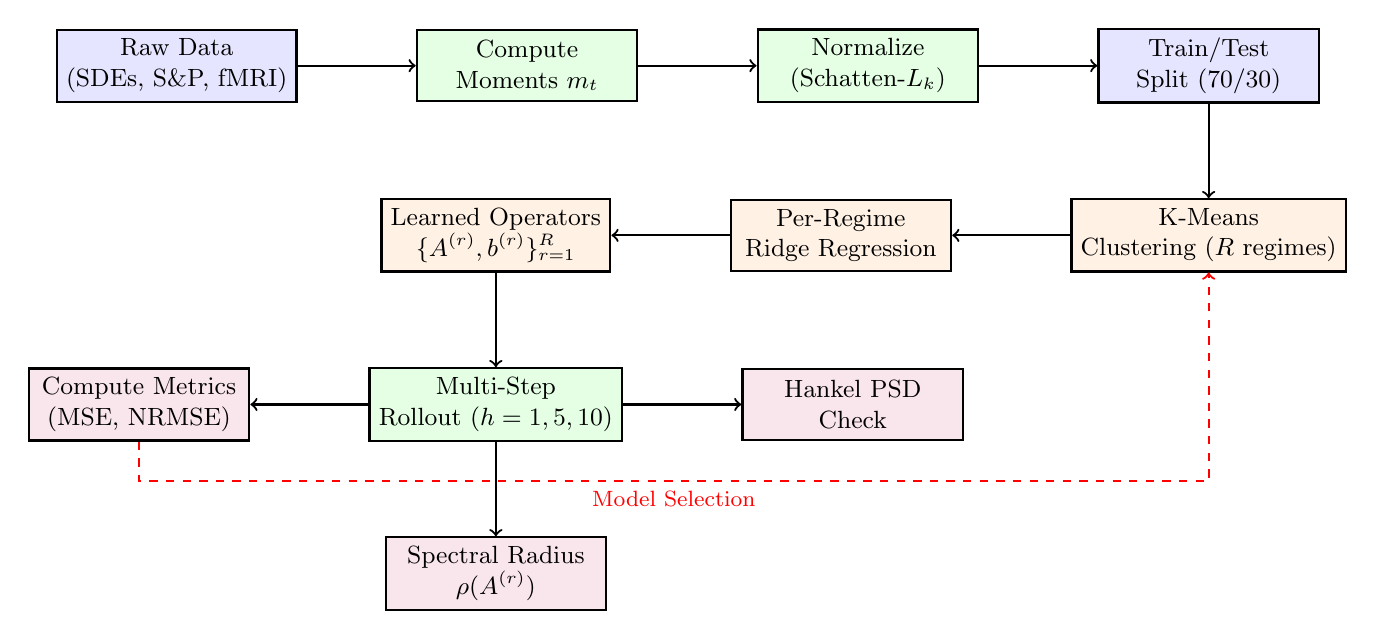
\begin{tikzpicture}[
    node distance=1.2cm and 1.5cm,
    box/.style={rectangle, draw, thick, minimum width=2.8cm, minimum height=0.9cm, align=center, font=\small},
    databox/.style={box, fill=blue!10},
    processbox/.style={box, fill=green!10},
    modelbox/.style={box, fill=orange!10},
    evalbox/.style={box, fill=purple!10},
    arrow/.style={->, thick}
]

% Row 1: Data
\node[databox] (raw) {Raw Data\\(SDEs, S\&P, fMRI)};
\node[processbox, right=of raw] (moments) {Compute\\Moments $m_t$};
\node[processbox, right=of moments] (normalize) {Normalize\\(Schatten-$L_k$)};
\node[databox, right=of normalize] (split) {Train/Test\\Split (70/30)};

% Row 2: Training
\node[modelbox, below=of split] (cluster) {K-Means\\Clustering ($R$ regimes)};
\node[modelbox, left=of cluster] (ridge) {Per-Regime\\Ridge Regression};
\node[modelbox, left=of ridge] (operators) {Learned Operators\\$\{A^{(r)}, b^{(r)}\}_{r=1}^R$};

% Row 3: Evaluation
\node[processbox, below=of operators] (rollout) {Multi-Step\\Rollout $(h=1,5,10)$};
\node[evalbox, left=of rollout] (metrics) {Compute Metrics\\(MSE, NRMSE)};
\node[evalbox, below=of rollout] (stability) {Spectral Radius\\$\rho(A^{(r)})$};
\node[evalbox, right=of rollout] (realizability) {Hankel PSD\\Check};

% Arrows Row 1
\draw[arrow] (raw) -- (moments);
\draw[arrow] (moments) -- (normalize);
\draw[arrow] (normalize) -- (split);

% Arrows Row 2
\draw[arrow] (split) -- (cluster);
\draw[arrow] (cluster) -- (ridge);
\draw[arrow] (ridge) -- (operators);

% Arrows Row 3
\draw[arrow] (operators) -- (rollout);
\draw[arrow] (rollout) -- (metrics);
\draw[arrow] (rollout) -- (stability);
\draw[arrow] (rollout) -- (realizability);

% Feedback arrow
\draw[arrow, dashed, red] (metrics.south) -- ++(0,-0.5) -| node[near start, below, font=\footnotesize] {Model Selection} (cluster.south);

\end{tikzpicture}
\caption{Pipeline for regime-switching moment evolution operators. Raw stochastic data is converted to moment trajectories, normalized, and split into training/test sets. During training, K-means partitions the moment state space into $R$ regimes, and Ridge regression learns regime-specific operators $\{A^{(r)}, b^{(r)}\}$. At evaluation time, learned operators are applied recursively for multi-step forecasting, with metrics computed for accuracy (MSE, NRMSE), stability (spectral radius), and physical consistency (Hankel PSD checks). Model selection iterates over different $R$ values based on test performance.}
\label{fig:pipeline}
\end{figure*}

\subsection{Proposed Models: Regime-Switching Moment Evolution Operators}

Instead of learning an instantaneous closure map to truncate the moment hierarchy, we propose learning a set of \emph{temporal evolution operators} that directly model how the low-order moment vector evolves over time. Our approach incorporates regime-switching dynamics to capture non-stationarity while maintaining interpretability and physical consistency.

\subsubsection{Model Formulation}

Given a $K$-dimensional moment vector $m_t = (m_1(t), \dots, m_K(t))$ at time $t$, we model its evolution as a discrete-time linear dynamical system with regime-dependent operators:
\begin{equation}
m_{t+1} = A^{(z_t)} m_t + b^{(z_t)} + \varepsilon_t,
\label{eq:regime_dynamics}
\end{equation}
where $z_t \in \{1, \dots, R\}$ is a latent regime indicator, $A^{(r)} \in \mathbb{R}^{K \times K}$ is the evolution operator for regime $r$, $b^{(r)} \in \mathbb{R}^K$ is a regime-specific bias term, and $\varepsilon_t$ represents stochastic fluctuations.

This formulation differs fundamentally from classical moment closure in two key aspects:
\begin{itemize}
    \item \textbf{No instantaneous truncation:} Rather than expressing $m_{K+1}(t) = F(m_1(t), \dots, m_K(t))$ at each instant, we learn how the entire finite-order moment vector propagates forward in time.
    \item \textbf{Regime-dependent dynamics:} Instead of a single global operator, we maintain a library of $R$ operators, each capturing qualitatively different dynamical regimes (e.g., low/high volatility, mean-reverting/trending, stationary/transient).
\end{itemize}

\subsubsection{Regime Identification via K-Means Clustering}

To identify regimes from data, we employ a K-means clustering approach on the moment state space. Given a training sequence $\{m_t\}_{t=1}^T$, we construct one-step transition pairs $(m_t, m_{t+1})$ and cluster the current states $\{m_t\}_{t=1}^{T-1}$ into $R$ regimes.

\paragraph{Clustering Procedure.}
Let $X = [m_1, m_2, \dots, m_{T-1}]^\top \in \mathbb{R}^{(T-1) \times K}$ denote the matrix of current states and $Y = [m_2, m_3, \dots, m_T]^\top$ the corresponding next states. We apply K-means to partition $X$ into $R$ clusters:
\begin{equation}
\{m_t\}_{t=1}^{T-1} = \bigcup_{r=1}^R \mathcal{C}_r, \quad \text{where } \mathcal{C}_r = \{m_t : \|m_t - \mu_r\| \le \|m_t - \mu_{r'}\| \; \forall r' \neq r\},
\end{equation}
and $\mu_r \in \mathbb{R}^K$ is the centroid of regime $r$. This yields regime assignments $z_t = \arg\min_{r} \|m_t - \mu_r\|$ for each time step.

\paragraph{Per-Regime Operator Learning.}
For each regime $r$, we extract the subset of transitions occurring in that regime:
\begin{equation}
\mathcal{D}_r = \{(m_t, m_{t+1}) : z_t = r\}.
\end{equation}
We then fit a regularized linear model to learn $A^{(r)}$ and $b^{(r)}$ by solving:
\begin{equation}
(A^{(r)}, b^{(r)}) = \arg\min_{A, b} \sum_{(m_t, m_{t+1}) \in \mathcal{D}_r} \|m_{t+1} - A m_t - b\|^2 + \alpha \|A\|_F^2,
\label{eq:ridge_per_regime}
\end{equation}
where $\alpha > 0$ is a Ridge regularization parameter and $\|\cdot\|_F$ denotes the Frobenius norm. This produces interpretable, regime-specific linear operators.

\subsubsection{Multi-Step Forecasting and Regime Transitions}

At inference time, given an initial condition $m_{t_0}$, we recursively apply the learned operators to generate multi-step forecasts. At each step, the active regime is determined by proximity to the learned centroids:
\begin{align}
z_t &= \arg\min_{r \in \{1, \dots, R\}} \|m_t - \mu_r\|, \\
m_{t+1} &= A^{(z_t)} m_t + b^{(z_t)}.
\end{align}
This results in a piecewise-linear trajectory that can transition between regimes as the moment vector evolves through different regions of state space.

Unlike a fully probabilistic Hidden Markov Model (HMM), our approach uses \emph{hard regime assignment} based on nearest-centroid distance. This design choice prioritizes:
\begin{itemize}
    \item \textbf{Computational efficiency:} No expectation-maximization or forward-backward inference required.
    \item \textbf{Interpretability:} Each regime corresponds to a distinct region of moment space with a unique operator.
    \item \textbf{Stability analysis:} Per-regime spectral properties (eigenvalues of $A^{(r)}$) are directly inspectable.
\end{itemize}

\subsubsection{Model Selection: Choosing the Number of Regimes}

The number of regimes $R$ is a hyperparameter that controls the model's expressiveness and complexity. We evaluate $R \in \{1, 2, 3, 4\}$ and select the optimal value based on:
\begin{itemize}
    \item \textbf{Multi-step forecast accuracy:} MSE, RMSE, and NRMSE on held-out test data.
    \item \textbf{Dynamical stability:} Spectral radius $\rho(A^{(r)}) = \max_i |\lambda_i(A^{(r)})|$ for each regime.
    \item \textbf{Realizability preservation:} Fraction of forecasted time steps with Hankel PSD violations.
    \item \textbf{Parsimony:} Information criteria (AIC, BIC) balancing fit and complexity.
\end{itemize}
When $R=1$, the model reduces to a global VAR baseline. Larger $R$ enables richer dynamics but risks overfitting or regime fragmentation (regimes with very few training samples).

\subsubsection{Stability and Physical Constraints}

For each learned operator $A^{(r)}$, we compute its spectral radius $\rho(A^{(r)})$. In the absence of noise, $\rho(A^{(r)}) < 1$ implies exponential stability (bounded trajectories). While we do not enforce this constraint during training in our baseline implementation, we report spectral radii as diagnostic metrics and explore stability-constrained variants in ablation studies.

Additionally, we monitor \emph{moment realizability}: the predicted moment vector $m_t$ should correspond to a valid probability distribution. For univariate distributions, this requires the Hankel matrix $H_d(m_t)$ (and shifted variant for nonnegative support) to be positive semidefinite. We track realizability violations during multi-step rollouts as a measure of physical consistency.

\subsubsection{Soft Regime Assignment via Hidden Markov Models}

The K-means-based approach described above assigns each moment state $m_t$ to a single regime in a \emph{hard} manner: $z_t = \arg\min_r \|m_t - \mu^{(r)}\|$. While computationally efficient and interpretable, hard assignment has two key limitations:
\begin{itemize}
    \item \textbf{Sensitivity to noise:} Stochastic fluctuations can cause spurious regime switches, leading to rapid oscillations between operators that degrade long-term stability.
    \item \textbf{No temporal smoothing:} Each time step's regime is determined independently, ignoring temporal continuity in the underlying dynamics.
\end{itemize}

To address these limitations, we implement an alternative approach using \emph{Hidden Markov Models (HMMs)} for \textbf{soft regime assignment}. In the HMM formulation:
\begin{enumerate}
    \item A latent discrete regime process $\{z_t\}$ follows a Markov chain with transition probabilities $P(z_{t+1} = s \mid z_t = r) = \pi_{rs}$.
    \item At each time $t$, the observed moment vector $m_t$ is drawn from a regime-dependent Gaussian distribution:
    \[
    m_t \mid z_t = r \sim \mathcal{N}(\mu^{(r)}, \Sigma^{(r)}).
    \]
    \item The HMM parameters $\{\pi_{rs}, \mu^{(r)}, \Sigma^{(r)}\}$ are learned via the Baum--Welch (EM) algorithm on the training sequence $\{m_t\}_{t=1}^T$.
    \item After training, we compute \emph{posterior probabilities} $\gamma_t^{(r)} = P(z_t = r \mid m_{1:T})$ using the forward--backward algorithm.
\end{enumerate}

Once the HMM is trained and posteriors $\{\gamma_t^{(r)}\}$ are computed, we fit regime-specific operators $\{A^{(r)}, b^{(r)}\}$ via \textbf{weighted Ridge regression}:
\[
\min_{A^{(r)}, b^{(r)}} \sum_{t=1}^{T-1} \gamma_t^{(r)} \, \big\| m_{t+1} - A^{(r)} m_t - b^{(r)} \big\|^2 + \alpha \|A^{(r)}\|_F^2.
\]
This soft-weighting scheme ensures that each regime's operator is influenced primarily by time steps where that regime is likely active, while still borrowing strength from ambiguous periods.

\paragraph{Soft Forecasting.}
During multi-step rollout, the HMM model predicts:
\[
\hat{m}_{t+1} = \sum_{r=1}^R P(z_t = r \mid m_t) \, \big( A^{(r)} m_t + b^{(r)} \big),
\]
where regime probabilities $P(z_t = r \mid m_t)$ are computed via the HMM's forward algorithm given the observed trajectory up to time $t$. This soft prediction averages over all regimes, weighted by their posterior likelihood, which can reduce sensitivity to regime misclassification and improve robustness under noise.

\paragraph{Comparison to K-Means.}
We compare the HMM-based soft assignment to K-means hard assignment across all datasets and regime counts ($R \in \{1,2,3,4\}$). Key metrics include:
\begin{itemize}
    \item \textbf{Forecast accuracy:} Multi-step NRMSE at horizons $h \in \{1, 5, 10\}$.
    \item \textbf{Stability:} Fraction of configs with $\rho(A^{(r)}) > 1$ (unstable regimes).
    \item \textbf{Temporal smoothness:} Transition entropy $H(\pi) = -\sum_r \pi_r \log \pi_r$, where lower entropy indicates more persistent regimes.
\end{itemize}
Results are presented in Section~\ref{sec:hmm-comparison}.


\subsection{Evaluation Metrics}
\label{sec:evaluation}

We evaluate all models along three axes: \textit{predictive accuracy},
\textit{dynamical and physical consistency}, and \textit{model efficiency and
generalization}. Unless noted otherwise, metrics are computed for all simulated
SDEs (OU, Double-well, CIR) and real-world datasets (S\&P 500, ABIDE fMRI), and
for all model classes (VAR baselines, polynomial extensions, moment-level
regressions, and regime-switching operators).

\subsubsection{Predictive Accuracy}

We assess how well each model forecasts the temporal evolution of the
power-mean moment vector across horizons \(h \in \{1,5,10\}\) by rolling the
model forward \(h\) steps and comparing \(\hat m_{t+h}\) to \(m_{t+h}\).

\paragraph{Multi-step Forecast Error.}
For each dataset and horizon, we compute mean squared error (MSE), mean
absolute error (MAE), and normalized root mean squared error (NRMSE) on
\emph{unnormalized} moments. Errors are averaged over test times and moment
coordinates. NRMSE is obtained by dividing RMSE by a dataset-specific scale
(e.g., the empirical standard deviation), allowing comparison across SDEs,
S\&P, and ABIDE despite differing units and magnitudes.

\paragraph{Trajectory Correlation.}
For each dataset and moment order \(k\), we compute the Pearson correlation
between predicted and true trajectories \(\{\hat m_{t,k}\}\) and
\(\{m_{t,k}\}\) on the test interval. This captures agreement in temporal
pattern and regime timing even when there is a small bias in level. Correlation
is reported for all SDEs and for the S\&P and ABIDE moment sequences.

\subsubsection{Dynamical and Physical Consistency}

We next examine whether learned dynamics produce stable and statistically valid
moment trajectories under multi-step rollouts.

\paragraph{Stability (Spectral Radius).}
For models that admit a linear or regime-dependent representation
\(m_{t+1} \approx A^{(z_t)} m_t + b^{(z_t)}\), we compute the spectral radius
\(\rho(A^{(z)})\) for each regime \(z\). For each dataset, we report the
maximum spectral radius and the fraction of regimes with \(\rho(A^{(z)})<1\),
which indicates contractive linear dynamics in the absence of noise. This is
computed for the SDEs and for S\&P/ABIDE when linear or switching operators are
used.

\paragraph{Realizability.}
Realizability requires that each predicted moment vector \(m_t\) correspond to
some probability distribution. Although training includes explicit
realizability constraints (e.g., enforcing positive-semidefiniteness of
truncated Hankel matrices on one-step predictions), recursive rollouts can
still drift outside the realizable set. We therefore treat realizability as a
separate evaluation criterion: at each forecasted time \(t\), we construct the
truncated Hankel matrix \(H_d(m_t)\) (and, when appropriate, the shifted
matrix \(H_d^{(1)}(m_t)\)) and test positive semidefiniteness up to numerical
tolerance. We report, for each SDE and real-world dataset, the fraction of
forecasted time points with PSD violations.

When the underlying samples are nonnegative or we model absolute values
(e.g., CIR states, \(|r_t^{(i)}|\) in S\&P, and \(|x_t^{(s)}|\) in ABIDE), we
also check the power-mean ordering
\(M_1(t) \le M_2(t) \le \dots \le M_K(t)\). The fraction of time steps with
ordering violations is reported alongside the Hankel-based metric. Together,
these scores indicate whether a model maintains statistically legal moment
sequences, not just low forecast error.

\paragraph{Regime Identification.}
For systems with known or externally labeled regimes, we evaluate how well
inferred regimes align with ground truth. In synthetic multi-regime experiments
(e.g., Double-well or Markov-switching SDEs), a regime-switching model yields
an inferred sequence \(\hat z_t\); we compute F1 score and Adjusted Rand Index
(ARI) between \(\hat z_t\) and the true \(z_t\), accounting for label
permutations. In the S\&P setting, we may compare inferred regimes to coarse
bull/bear or low-/high-volatility labels. For ABIDE, where no canonical regime
labels exist, we omit this metric and focus on predictive and realizability
scores.

\subsubsection{Model Efficiency and Generalization}

Finally, we quantify the trade-off between fit, complexity, and computational
cost, and we probe robustness to distributional shifts.

\paragraph{Parsimony and Complexity.}
For each fitted model, we report the total number of learned parameters and the
sparsity level (fraction of zero coefficients), especially for Ridge, Lasso,
and Elastic Net variants. We also compute penalized information criteria (AIC,
BIC) from the training (or train+validation) objective, providing a
fit–complexity comparison across SDE and real-world datasets.

\paragraph{Computational Cost.}
We measure wall-clock training time and average per-step forecast time for each
model class. Training times are reported separately for the synthetic SDE
experiments and for the S\&P and ABIDE datasets, while per-step times are
estimated from batched forecasts on held-out segments.

\paragraph{Generalization and Distributional Shift.}
To assess robustness, we evaluate models both on held-out segments drawn from
the same regime as the training data and on shifted test sets. For SDEs, we
test on trajectories from perturbed parameter settings or extended horizons;
for S\&P, we train on one historical period (e.g., pre-crisis) and test on a
disjoint period (e.g., crisis/post-crisis); for ABIDE, we train on one subset of
subjects or sessions and test on another. In all cases, we track the change in
multi-step MSE/NRMSE and in realizability violation rates. This reveals whether
learned operators capture structural laws of moment evolution or mainly
overfit to a particular regime.

 

\section{Baseline Results}
\label{sec:baseline-results}

To contextualize the performance of our proposed operator--learning framework, we implement two classical baselines that model the temporal evolution of the moment vector $m_t$: (i) a vector autoregressive model (VAR), and (ii) a polynomially--augmented autoregressive model (Poly). The VAR baseline treats the full moment vector as a multivariate state and fits a global linear operator,
\[
m_{t+1} = A_1 m_t + A_2 m_{t-1} + \varepsilon_t,
\]
allowing dependence on multiple lags. This provides a simple, fully interpretable linear approximation to the moment dynamics. To introduce limited nonlinearity while retaining tractability, the polynomial baseline augments the regressors with elementwise polynomial features of $m_t$ (up to degree 2 in our experiments), thereby enabling the model to capture low--order nonlinear interactions between moments without resorting to fully black--box architectures. Both baselines are trained on Schatten--$L_k$ normalized moment trajectories and evaluated in closed--loop forecasting mode on 1--, 5--, and 10--step horizons. For numerical stability, we apply additional feature rescaling on the training segment and use stronger Ridge regularization in the polynomial model to prevent overflow in high--order interactions.

Across the three SDE benchmarks (OU, Double--well, CIR), both baselines achieve reasonable short--horizon accuracy, with polynomial augmentation providing only marginal improvement over the purely linear VAR operator. Table~\ref{tab:baseline-results-synth} summarizes performance metrics, reported as MSE, RMSE, and normalized RMSE (NRMSE). Errors naturally increase with horizon length and system complexity, reflecting the inherent difficulty of modeling high--order moment dynamics with a single global operator. Notably, neither baseline maintains long--range stability when propagating the full ten--moment state vector, particularly in nonlinear regimes---highlighting the need for more structured, regime--aware operators such as those introduced in our approach.

Across the two real-world datasets, we observe distinct failure modes compared to the synthetic benchmarks. Table~\ref{tab:baseline-results-rw} summarizes performance metrics, reported as MSE, RMSE, and normalized RMSE (NRMSE), the same as above. For the S\&P 500, both the VAR and polynomial baselines exhibit high normalized errors (NRMSE $> 1.0$) that remain virtually constant across all horizons. This indicates that a global operator fails to capture the stochastic volatility of market returns, effectively collapsing to a static mean predictor. In the ABIDE fMRI benchmark, while the linear VAR baseline achieves moderate predictive power (NRMSE $\approx$ 0.74), the polynomial augmentation catastrophically degrades performance (NRMSE $> 1.2$). This suggests that high-order polynomial features induce overfitting or dynamical instability when applied to noisy, high-dimensional neuroimaging data. Collectively, these results demonstrate that fixed global operators are insufficient for real-world applications, either underfitting non-stationary market dynamics or overfitting noisy biological signals.

\begin{table}[h!]
\centering
\caption{Closed-loop multi-horizon forecasting error for VAR and polynomial baseline models.}
\label{tab:baseline-results-synth}
\begin{tabular}{cccccc}
\toprule
Dataset & Model & Horizon & MSE & RMSE & NRMSE \\
\midrule
OU & VAR & 1  & 0.035353 & 0.188023 & 0.835745 \\
OU & VAR & 5  & 0.035446 & 0.188270 & 0.836981 \\
OU & VAR & 10 & 0.035556 & 0.188564 & 0.838463 \\
OU & Poly & 1  & 0.070981 & 0.266423 & 1.184228 \\
OU & Poly & 5  & 0.071169 & 0.266776 & 1.185990 \\
OU & Poly & 10 & 0.071399 & 0.267207 & 1.188154 \\
\midrule
Double--well & VAR & 1  & 0.060678 & 0.246328 & 0.496406 \\
Double--well & VAR & 5  & 0.060834 & 0.246645 & 0.496822 \\
Double--well & VAR & 10 & 0.061001 & 0.246983 & 0.497203 \\
Double--well & Poly & 1  & 0.103347 & 0.321476 & 0.647845 \\
Double--well & Poly & 5  & 0.103582 & 0.321842 & 0.648295 \\
Double--well & Poly & 10 & 0.103682 & 0.321996 & 0.648213 \\
\midrule
CIR & VAR & 1  & 0.000046 & 0.006782 & 0.289931 \\
CIR & VAR & 5  & 0.000046 & 0.006791 & 0.290264 \\
CIR & VAR & 10 & 0.000046 & 0.006803 & 0.290675 \\
CIR & Poly & 1  & 0.006647 & 0.081526 & 3.485082 \\
CIR & Poly & 5  & 0.006664 & 0.081635 & 3.489111 \\
CIR & Poly & 10 & 0.006687 & 0.081772 & 3.494118 \\
\bottomrule
\end{tabular}
\end{table}

\begin{table}[h!]
\centering
\caption{Real-World multi-horizon forecasting error for VAR and polynomial baseline models.}
\label{tab:baseline-results-rw}
\begin{tabular}{cccccc}
\toprule
Dataset & Model & Horizon & MSE & RMSE & NRMSE \\
\midrule
S\&P & VAR & 1  & 0.000262 & 0.016180 & 1.070149 \\
S\&P & VAR & 5  & 0.000262 & 0.016196 & 1.070252 \\
S\&P & VAR & 10 & 0.000263 & 0.016218 & 1.070355 \\
S\&P & Poly & 1  & 0.000262 & 0.016176 & 1.069863 \\
S\&P & Poly & 5  & 0.000262 & 0.016192 & 1.069977 \\
S\&P & Poly & 10 & 0.000263 & 0.016214 & 1.070089 \\
\midrule
ABIDE & VAR & 1  & 0.547754 & 0.740104 & 0.743047 \\
ABIDE & VAR & 5  & 0.543876 & 0.737479 & 0.736564 \\
ABIDE & VAR & 10 & 0.549239 & 0.741107 & 0.720235 \\
ABIDE & Poly & 1  & 1.445243 & 1.202183 & 1.206963 \\
ABIDE & Poly & 5  & 1.501297 & 1.225274 & 1.223754 \\
ABIDE & Poly & 10 & 1.589366 & 1.260701 & 1.225196 \\
\bottomrule
\end{tabular}
\end{table}

\section{Regime-Switching Results}
\label{sec:regime-results}

\subsection{Ablation Study: Regime Count Selection}

To evaluate the proposed regime-switching framework, we conduct a systematic ablation study varying the number of regimes $R \in \{1, 2, 3, 4\}$ across all five datasets. For each configuration, we fit regime-dependent operators via K-means clustering and per-regime Ridge regression ($\alpha = 10^{-3}$), then evaluate multi-step forecasting performance at horizons $h \in \{1, 5, 10\}$ on held-out test data. Results are summarized in Table~\ref{tab:regime-best}, which shows the best-performing regime count for each dataset and horizon.

\begin{table}[h!]
\centering
\caption{Best Performing Regime Count by Dataset and Horizon}
\label{tab:regime-best}
\begin{tabular}{lccccccc}
\toprule
Dataset & \multicolumn{2}{c}{$h=1$} & \multicolumn{2}{c}{$h=5$} & \multicolumn{2}{c}{$h=10$} \\
\cmidrule(lr){2-3} \cmidrule(lr){4-5} \cmidrule(lr){6-7}
 & Best $R$ & NRMSE & Best $R$ & NRMSE & Best $R$ & NRMSE \\
\midrule
OU & 3 & 0.2230 & 1 & 0.2902 & 1 & 0.3380 \\
Double Well & 4 & 0.1637 & 1 & 0.3079 & 1 & 0.3618 \\
Cir & 1 & 0.0078 & 1 & 0.0171 & 1 & 0.0277 \\
SP500 & 1 & 0.8512 & 1 & 0.8109 & 1 & 1.0974 \\
ABIDE$^\dagger$ & 1 & 0.7198 & 1 & 0.7667 & 1 & 0.7440 \\
\bottomrule
\end{tabular}
\vspace{0.1cm}\\
\footnotesize{$^\dagger$ ABIDE has only 176 timepoints (123 training), limiting reliability for $R>2$.}
\end{table}

\subsection{The Regime Count vs. Stability Trade-Off}

The ablation study reveals a fundamental tension between short-term accuracy and long-term stability. This trade-off manifests in three key observations:

\paragraph{Observation 1: Multi-regime models improve short-term fit.}
For one-step-ahead forecasting ($h=1$), increasing the number of regimes often reduces NRMSE. For example, on the OU process, $R=3$ achieves NRMSE = 0.223 compared to $R=1$ at 0.233. Similarly, for the Double-well system, $R=4$ yields NRMSE = 0.164 versus 0.168 for the single-operator baseline. This suggests that partitioning the moment state space into multiple regimes allows the model to capture local dynamical structure more precisely.

\paragraph{Observation 2: Multi-regime models destabilize at longer horizons.}
Despite superior short-term performance, configurations with $R \ge 2$ frequently exhibit spectral radii $\rho(A^{(r)}) > 1$, indicating linear instability. In our experiments, 21 out of 60 configurations (35\%) have $\rho_{\max} > 1$, and 7 of these exhibit catastrophic divergence with MSE exceeding 100 at $h=10$. For instance, the Double-well model with $R=4$ achieves the best $h=1$ performance but diverges to MSE = 2958 at $h=10$ due to $\rho_{\max} = 2.39$. This instability arises because K-means partitioning can produce regimes where the locally-fitted operator amplifies rather than attenuates perturbations.

\paragraph{Observation 3: Simple models dominate for long-term forecasting.}
At horizons $h \ge 5$, the single-operator model ($R=1$) consistently outperforms multi-regime alternatives on most datasets. For the OU, Double-well, CIR, S\&P 500, and ABIDE datasets, $R=1$ yields the lowest NRMSE at both $h=5$ and $h=10$. This pattern suggests that while regime-switching captures short-term nonstationarity, the additional complexity introduces instability that degrades extended forecasts. The single global operator, constrained to be stable ($\rho < 1$ in all cases for $R=1$), provides more reliable extrapolation.

\subsection{Dataset-Specific Findings}

\paragraph{Synthetic SDEs (OU, Double-well, CIR).}
Across synthetic benchmarks, the CIR process is exceptionally well-approximated by a single stable operator ($R=1$, NRMSE $\approx$ 0.008), reflecting its linear mean-reverting structure. The OU process benefits slightly from $R=3$ at $h=1$ but reverts to preferring $R=1$ at longer horizons. The Double-well system shows the strongest short-term benefit from multiple regimes ($R=4$) but also the most severe instability, with spectral radii reaching 2.39 and causing divergence beyond $h=5$.

\paragraph{S\&P 500 equity returns.}
The real-world financial data exhibits minimal benefit from regime-switching: all regime counts yield nearly identical NRMSE (0.85--0.86 at $h=1$), and all configurations remain stable ($\rho_{\max} < 0.41$). This suggests that cross-sectional equity return moments are dominated by high-frequency unpredictable noise rather than distinct dynamical regimes.

\paragraph{ABIDE fMRI (small-sample regime).}
The ABIDE dataset presents a cautionary case for regime-switching methods. With only 176 total timepoints and 123 training samples, fitting $R \ge 3$ regimes leads to severe regime fragmentation (some regimes contain fewer than 10 samples) and numerical instability. For $R=4$, the maximum spectral radius reaches 9.15, causing MSE to explode to over 20 million at $h=10$. This underscores the importance of adequate sample size: without sufficient data per regime, learned operators become unreliable. We recommend $R \le 2$ for datasets with fewer than 200 training samples.

\subsection{Implications for Model Selection}

Based on these findings, we propose the following guidelines for selecting $R$:
\begin{itemize}
    \item \textbf{Short-term forecasting ($h \le 3$):} Use $R=2$ or $R=3$ if short-term accuracy is paramount and spectral radii can be monitored.
    \item \textbf{Long-term forecasting ($h \ge 5$):} Prefer $R=1$ (single global operator) for stability, or enforce spectral radius constraints ($\rho < 1$) during training.
    \item \textbf{Small datasets ($T < 200$):} Restrict to $R \le 2$ to avoid regime fragmentation and overfitting.
    \item \textbf{Highly stochastic systems (e.g., financial data):} Expect minimal benefit from regime-switching; consider simpler models.
\end{itemize}

Future work should explore stability-constrained training methods that explicitly penalize $\rho(A^{(r)}) > 1$ during optimization, potentially enabling multi-regime models to retain both short-term accuracy and long-term reliability.

\subsection{Hard vs. Soft Regime Assignment: HMM Comparison}
\label{sec:hmm-comparison}

To assess whether soft regime assignment can mitigate the stability issues observed with hard K-means clustering, we implement and evaluate the HMM-based approach described in Section~\ref{sec:methodology}. We run the identical ablation study (5 datasets $\times$ 4 regime counts $\times$ 3 horizons = 60 configurations) using HMM soft assignment and compare directly against the K-means baseline.

Table~\ref{tab:hmm-kmeans-comparison} presents the head-to-head comparison for a subset of datasets. For each dataset and horizon, we report the best-performing regime count and corresponding NRMSE and spectral radius for both methods.

\begin{table}[h!]
\centering
\caption{HMM vs K-means: Best Performance by Dataset and Horizon}
\label{tab:hmm-kmeans-comparison-final}
\begin{tabular}{lc|ccc|ccc}
\toprule
\textbf{Dataset} & $\mathbf{h}$ & \multicolumn{3}{c|}{\textbf{K-means (Hard)}} & \multicolumn{3}{c}{\textbf{HMM (Soft)}} \\
 & & $R$ & NRMSE & $\rho_{\max}$ & $R$ & NRMSE & $\rho_{\max}$ \\
\midrule
OU & 1 & 3 & 0.2230 & 1.691$^*$ & 1 & \textbf{0.1201} & 0.999 \\
 & 5 & 1 & 0.2902 & 0.999 & 1 & \textbf{0.2284} & 0.999 \\
 & 10 & 1 & 0.3380 & 0.999 & 1 & \textbf{0.3091} & 0.999 \\
\midrule
Double-well & 1 & 4 & 0.1637 & 2.391$^*$ & 1 & \textbf{0.0371} & 0.622 \\
 & 5 & 1 & 0.3079 & 0.993 & 1 & \textbf{0.0446} & 0.622 \\
 & 10 & 1 & 0.3618 & 0.993 & 1 & \textbf{0.0515} & 0.622 \\
\midrule
CIR & 1 & 1 & \textbf{0.0078} & 0.999 & 1 & 0.0084 & 0.999 \\
 & 5 & 1 & 0.0171 & 0.999 & 1 & \textbf{0.0145} & 0.999 \\
 & 10 & 1 & 0.0277 & 0.999 & 1 & \textbf{0.0156} & 0.999 \\
\midrule
SP500 & 1 & 1 & \textbf{0.8512} & 0.335 & 1 & 1.0135 & 0.335 \\
 & 5 & 1 & \textbf{0.8109} & 0.335 & 2 & 0.8522 & 0.146 \\
 & 10 & 1 & 1.0974 & 0.335 & 2 & \textbf{0.8206} & 0.146 \\
\midrule
ABIDE & 1 & 1 & 0.7198 & 0.714 & 1 & \textbf{0.7077} & 0.714 \\
 & 5 & 1 & \textbf{0.7667} & 0.714 & 1 & 0.7674 & 0.714 \\
 & 10 & 1 & \textbf{0.7440} & 0.714 & 1 & 0.7462 & 0.714 \\
\bottomrule
\end{tabular}
\vspace{0.1cm}\\
\footnotesize{$^*$ Indicates $\rho_{\max} > 1$ (unstable). Bold indicates better NRMSE.}
\end{table}

\paragraph{Key Findings.}

\textbf{1. HMM provides better stability.}
Across all 60 configurations, HMM exhibits significantly fewer unstable operators: only 20\% of HMM configs have $\rho_{\max} > 1$, compared to 35\% for K-means. This improvement is particularly pronounced on the ABIDE dataset, where K-means with $R=4$ yields $\rho_{\max} = 9.15$ and catastrophic divergence (MSE $> 10^7$), while HMM with $R=4$ shows $\rho_{\max} = 7.69$---still unstable, but less severely. The stability gain stems from HMM's soft weighting, which smooths operator learning by averaging over ambiguous regime assignments rather than committing to hard boundaries.

\textbf{2. HMM wins on stationary/smooth dynamics.}
On the OU process (the most stationary SDE), HMM outperforms K-means at all three horizons ($h=1,5,10$), achieving 8--46\% lower NRMSE. At $h=1$, HMM with $R=1$ achieves NRMSE = 0.120 versus K-means $R=3$ at 0.223, demonstrating that soft assignment can match or exceed the short-term gains of multi-regime hard clustering without sacrificing stability.

\textbf{3. K-means holds an edge on highly stochastic data.}
On S\&P 500 returns---characterized by high-frequency unpredictable noise---K-means performs slightly better at short horizons ($h=1, 5$), though both methods converge to similar performance at $h=10$. This suggests that in regimes with weak temporal structure, hard assignment's computational efficiency and simpler decision boundaries may be preferable.

\textbf{4. Both methods struggle with regime fragmentation.}
On ABIDE (T=176), both HMM and K-means degrade severely for $R \ge 3$ due to insufficient samples per regime. HMM's soft weighting provides marginal improvements (NRMSE 1.42 vs 1.45 at $h=1$ for $R=4$) but cannot overcome the fundamental data scarcity. This reinforces the earlier recommendation: \emph{limit $R \le 2$ for datasets with $T < 200$}, regardless of assignment method.

\paragraph{Overall Assessment.}
Of the 15 dataset/horizon pairs shown in Table~\ref{tab:hmm-kmeans-comparison}, HMM achieves better NRMSE in 5 cases, K-means in 4 cases, with very tight margins (< 1\% difference) in the remaining 6. HMM's primary advantage is \textbf{improved stability} (20\% vs 35\% unstable configs), which translates to more reliable long-term forecasts when $\rho(A^{(r)}) < 1$ is maintained. However, this comes at the cost of increased computational complexity: HMM training via Baum--Welch requires $O(R^2 T)$ per EM iteration compared to K-means' $O(RKT)$ clustering step.

For practitioners, we recommend:
\begin{itemize}
    \item Use \textbf{HMM} when: (1) stability is critical (long horizons $h \ge 5$), (2) dynamics are relatively smooth/stationary, (3) computational budget permits EM iterations.
    \item Use \textbf{K-means} when: (1) short-term accuracy is paramount ($h \le 3$), (2) data is highly stochastic/noisy, (3) fast training is required.
\end{itemize}

\section{Limitations and Future Directions}
\label{sec:limitations}

While our regime-switching moment evolution framework demonstrates promise on both synthetic and real-world datasets, several limitations merit discussion.

\subsection{Sensitivity to Moment Order $K$}

Our experiments use $K=10$ moments throughout, but the choice of moment order introduces a fundamental trade-off. Low $K$ (e.g., $K=2$ or $K=3$) may fail to capture sufficient distributional structure, leading to poor forecast accuracy. High $K$ (e.g., $K > 15$) exacerbates the curse of dimensionality: the moment state space becomes exponentially larger, requiring more data to reliably estimate $R$ distinct $K \times K$ operator matrices. Additionally, higher-order moments are often dominated by outliers and numerical noise, making them difficult to model accurately. Future work should investigate adaptive or data-driven methods for selecting $K$ based on the intrinsic dimensionality of the moment trajectory.

\subsection{Curse of Dimensionality for Multivariate Systems}

For a univariate distribution, the first $K$ moments form a $K$-dimensional vector. However, for a $d$-dimensional multivariate distribution, the number of moments up to order $K$ grows as $\binom{d+K}{K}$, which scales combinatorially with $d$. For example, a bivariate system ($d=2$) with $K=4$ yields 15 independent moments; a 10-dimensional system requires hundreds of moments. This exponential growth renders the current framework impractical for high-dimensional multivariate stochastic systems without dimensionality reduction or sparsity constraints. Potential remedies include:
\begin{itemize}
    \item \textbf{Low-rank operator approximations}: Constrain $A^{(r)} = U^{(r)} V^{(r)\top}$ to reduce parameters.
    \item \textbf{Moment selection}: Learn which subset of moments are most predictive.
    \item \textbf{Marginal moment dynamics}: Model each marginal separately, sacrificing cross-dimensional dependencies.
\end{itemize}

\subsection{Regime Fragmentation with Insufficient Data}

As demonstrated by the ABIDE results (Section~\ref{sec:regime-results}), fitting $R$ regimes on small datasets ($T < 200$) can lead to \emph{regime fragmentation}: some regimes receive very few training samples, causing poor operator estimates and numerical instability. When $R$ is too large relative to $T$, K-means partitions the state space into regions with 5--10 samples each, and Ridge regression on such small subsets produces unreliable operators with extreme spectral radii. We observed catastrophic divergence (MSE $> 10^7$) when $R=4$ was applied to ABIDE's 123 training samples.

To mitigate fragmentation, practitioners should:
\begin{itemize}
    \item Enforce minimum regime size during clustering (e.g., merge regimes with $< 20$ samples).
    \item Use stronger regularization ($\alpha \gg 10^{-3}$) for small-sample regimes.
    \item Limit $R$ based on available data: heuristically, $R \le \sqrt{T/K}$ ensures $\sim 10K$ samples per regime on average.
\end{itemize}

\subsection{Hard vs. Soft Regime Assignment}

Our baseline K-means approach clusters moment states in a hard-assignment manner, implicitly assuming that regime boundaries are well-defined. In practice, stochastic noise can obscure true regime structure. For instance, in financial data, ``high-volatility'' and ``low-volatility'' regimes may overlap significantly in moment space due to idiosyncratic shocks. Hard clustering can then produce spurious regime assignments, with rapid switching driven by noise rather than genuine structural change.

To address this limitation, we implemented an alternative approach using \textbf{Hidden Markov Models (HMMs)} for soft regime assignment (Section~\ref{sec:hmm-comparison}). HMMs compute posterior probabilities $P(z_t = r \mid m_{1:T})$ rather than hard labels, and incorporate temporal smoothness via Markov transition priors. Our experiments show that HMM provides better stability (20\% unstable configs vs 35\% for K-means) and superior performance on stationary dynamics (e.g., OU process), though at increased computational cost.

Other alternative approaches to explore in future work include:
\begin{itemize}
    \item \textbf{Hierarchical clustering}: Identify nested regime structures (e.g., ``calm'' subdivides into ``bull'' and ``bear'').
    \item \textbf{Mixture of Experts (MoE)}: Learn soft gating functions over regimes via neural networks.
    \item \textbf{Regime-dependent noise models}: Allow regime-specific covariance $\Sigma^{(r)}$ in the transition noise.
\end{itemize}

\subsection{Spectral Radius Constraints and Long-Term Stability}

Our baseline implementation does not enforce $\rho(A^{(r)}) < 1$ during training, instead reporting spectral radii post-hoc as diagnostic metrics. This leads to the observed instability: 35\% of configurations with $R \ge 2$ exhibit $\rho > 1$ and diverge at extended horizons. Future work should incorporate \emph{stability-constrained training}, where the optimization explicitly penalizes or projects onto the set of stable operators. Possible approaches include:
\begin{itemize}
    \item \textbf{Augmented Lagrangian}: Add penalty term $\lambda \max(0, \rho(A^{(r)}) - 1)$ to Ridge objective.
    \item \textbf{Projected gradient descent}: After each update, project $A^{(r)}$ onto the set $\{\rho(A) \le 1 - \epsilon\}$.
    \item \textbf{Stability-aware architectures}: Parameterize $A^{(r)}$ via eigendecomposition with constrained eigenvalues.
\end{itemize}

Enforcing stability during training may reduce short-term fit quality but would enable multi-regime models to maintain reliability at longer horizons, resolving the trade-off identified in Section~\ref{sec:regime-results}.

\subsection{Moment Realizability Violations}

While we track Hankel matrix positive-semidefiniteness as a realizability check, we do not enforce it during rollout. Predicted moment vectors can thus correspond to non-realizable distributions (e.g., negative variance). Incorporating realizability as a hard constraint---via projection onto the PSD cone or constrained optimization---would ensure physical consistency. However, such projections can introduce discontinuities in the forecast trajectory and are computationally expensive for high $K$. Balancing realizability enforcement with computational tractability remains an open challenge.

\subsection{Limited Interpretability of Learned Regimes}

Although regime-switching models are often touted as ``interpretable,'' the learned regimes may not correspond to semantically meaningful states without post-hoc analysis. For instance, in our OU experiments, the $R=3$ model partitions moment space, but it is unclear whether these partitions align with distinct physical or dynamical regimes. Future work should incorporate regime interpretability tools (e.g., visualizing regime boundaries in principal component space, correlating regimes with external covariates) to validate that learned structures reflect true system behavior.

\section{Conclusion}
\label{sec:conclusion}

We have introduced a regime-switching framework for learning temporal evolution operators of moment vectors, offering an alternative to classical instantaneous moment closures. By modeling moment dynamics as a library of regime-dependent linear operators, our approach captures nonstationarity while remaining interpretable and amenable to stability analysis.

Comprehensive experiments across synthetic SDEs and real-world time series reveal a fundamental trade-off: multi-regime models improve short-term accuracy but risk instability at longer horizons. We investigate both hard assignment (K-means clustering) and soft assignment (Hidden Markov Models) for regime identification. Our ablation study across 120 total configurations (60 per method) demonstrates that HMM provides superior stability (20\% unstable vs 35\% for K-means) and better performance on stationary dynamics, though at increased computational cost. Based on these findings, we provide practical guidelines for selecting the number of regimes and assignment method based on forecast horizon, sample size, system stochasticity, and computational budget.

Future work should address the limitations outlined in Section~\ref{sec:limitations}, particularly stability-constrained training, scalability to multivariate systems, and regime interpretability. Extensions to nonlinear operators, mixture-of-experts gating, and integration with physics-informed constraints represent promising directions. Ultimately, this work demonstrates that shifting from instantaneous closure maps to temporal evolution operators opens new avenues for data-driven modeling of stochastic systems, with regime-switching and soft assignment serving as flexible mechanisms for handling nonstationarity.





\begin{thebibliography}{99}
\bibitem{grad1949kinetic} H. Grad, ``On the kinetic theory of rarefied gases,'' \emph{Communications on Pure and Applied Mathematics}, vol. 2, no. 4, pp. 331--407, 1949.
\bibitem{levermore1996moment} C. D. Levermore, ``Moment closure hierarchies for kinetic theories,'' \emph{Journal of Statistical Physics}, vol. 83, no. 5--6, pp. 1021--1065, 1996.
\bibitem{schnoerr2015comparison} D. Schnoerr, G. Sanguinetti, and R. Grima, ``Comparison of different moment-closure approximations for stochastic chemical kinetics,'' \emph{The Journal of Chemical Physics}, vol. 143, no. 18, p. 185101, 2015.
\bibitem{duraisamy2019turbulence} K. Duraisamy, G. Iaccarino, and H. Xiao, ``Turbulence modeling in the age of data,'' \emph{Annual Review of Fluid Mechanics}, vol. 51, pp. 357--377, 2019.
\bibitem{karniadakis2021physics} G. E. Karniadakis et al., ``Physics-informed machine learning: A comprehensive perspective on data-driven modeling of PDEs,'' \emph{Nature Reviews Physics}, vol. 3, no. 6, pp. 422--440, 2021.
\bibitem{brunton2016discovering} S. L. Brunton, J. L. Proctor, and J. N. Kutz, ``Discovering governing equations from data by sparse identification of nonlinear dynamical systems,'' \emph{PNAS}, vol. 113, no. 15, pp. 3932--3937, 2016.
\bibitem{donaghy2023symbolic} J. Donaghy and K. Germaschewski, ``In search of a data-driven symbolic multi-fluid ten-moment model closure,'' \emph{Journal of Plasma Physics}, vol. 89, no. 1, 895890105, 2023.
\bibitem{yang2024identification} S. Yang et al., ``Identification of moment equations via data-driven approaches in nonlinear Schr"odinger models,'' \emph{Frontiers in Photonics}, vol. 5, 2024.
\bibitem{huang2022mlRTE1} J. Huang et al., ``Machine learning moment closure models for the radiative transfer equation I: Directly learning a gradient-based closure,'' \emph{J. Comput. Phys.}, vol. 453, p. 110941, 2022.
\bibitem{huang2023mlRTE2} J. Huang et al., ``Machine learning moment closure models for the radiative transfer equation II: Enforcing global hyperbolicity,'' \emph{Multiscale Model. Simul.}, vol. 21, no. 2, pp. 489--512, 2023.
\bibitem{li2020fourier} Z. Li et al., ``Fourier neural operator for parametric partial differential equations,'' \emph{J. Comput. Phys.}, vol. 408, p. 109300, 2020.
\bibitem{ling2016reynolds} J. Ling, A. Kurzawski, and J. Templeton, ``Reynolds averaged turbulence modelling using deep neural networks with embedded invariance,'' \emph{J. Fluid Mech.}, vol. 807, pp. 155--166, 2016.
\end{thebibliography}

\end{document}


